\documentclass[a4paper]{article}\usepackage[]{graphicx}\usepackage[]{color}
% maxwidth is the original width if it is less than linewidth
% otherwise use linewidth (to make sure the graphics do not exceed the margin)
\makeatletter
\def\maxwidth{ %
  \ifdim\Gin@nat@width>\linewidth
    \linewidth
  \else
    \Gin@nat@width
  \fi
}
\makeatother

\definecolor{fgcolor}{rgb}{0.345, 0.345, 0.345}
\newcommand{\hlnum}[1]{\textcolor[rgb]{0.686,0.059,0.569}{#1}}%
\newcommand{\hlstr}[1]{\textcolor[rgb]{0.192,0.494,0.8}{#1}}%
\newcommand{\hlcom}[1]{\textcolor[rgb]{0.678,0.584,0.686}{\textit{#1}}}%
\newcommand{\hlopt}[1]{\textcolor[rgb]{0,0,0}{#1}}%
\newcommand{\hlstd}[1]{\textcolor[rgb]{0.345,0.345,0.345}{#1}}%
\newcommand{\hlkwa}[1]{\textcolor[rgb]{0.161,0.373,0.58}{\textbf{#1}}}%
\newcommand{\hlkwb}[1]{\textcolor[rgb]{0.69,0.353,0.396}{#1}}%
\newcommand{\hlkwc}[1]{\textcolor[rgb]{0.333,0.667,0.333}{#1}}%
\newcommand{\hlkwd}[1]{\textcolor[rgb]{0.737,0.353,0.396}{\textbf{#1}}}%
\let\hlipl\hlkwb

\usepackage{framed}
\makeatletter
\newenvironment{kframe}{%
 \def\at@end@of@kframe{}%
 \ifinner\ifhmode%
  \def\at@end@of@kframe{\end{minipage}}%
  \begin{minipage}{\columnwidth}%
 \fi\fi%
 \def\FrameCommand##1{\hskip\@totalleftmargin \hskip-\fboxsep
 \colorbox{shadecolor}{##1}\hskip-\fboxsep
     % There is no \\@totalrightmargin, so:
     \hskip-\linewidth \hskip-\@totalleftmargin \hskip\columnwidth}%
 \MakeFramed {\advance\hsize-\width
   \@totalleftmargin\z@ \linewidth\hsize
   \@setminipage}}%
 {\par\unskip\endMakeFramed%
 \at@end@of@kframe}
\makeatother

\definecolor{shadecolor}{rgb}{.97, .97, .97}
\definecolor{messagecolor}{rgb}{0, 0, 0}
\definecolor{warningcolor}{rgb}{1, 0, 1}
\definecolor{errorcolor}{rgb}{1, 0, 0}
\newenvironment{knitrout}{}{} % an empty environment to be redefined in TeX

\usepackage{alltt}
%\documentclass[gmd]{copernicus}
%\documentclass[article,nojss]{jss}
%\VignetteIndexEntry{ParameterEstimation}

%%%%%%%%%%%%%%%%%%%%%%%%%%%%%% Add-on packages and fonts
%\usepackage[utf8]{inputenc}
\usepackage{graphicx}
\usepackage{amsmath}

\usepackage{color}
\usepackage[round]{natbib}

%%%%%%%%%%%%%%%%%%%%%%%%%%%%%% User specified LaTeX commands.
%\newcommand{\R}{\proglang{R }}
\newcommand{\R}{\textsf{R }}
\newcommand{\SoilR}{\texttt{SoilR }}
\newcommand{\FME}{\texttt{FME }}
\newcommand{\GeneralModel}{\texttt{GeneralModel}}
\newcommand{\Model}{\texttt{Model}}
\newcommand{\BoundInFlux}{\texttt{BoundInFlux}}
\newcommand{\BoundLinDecompOp}{\texttt{BoundLinDecompOp}}
\newcommand{\ConstLinDecompOp}{\texttt{ConstLinDecompOp}}
\newcommand{\TimeMap}{\texttt{TimeMap}}
\newcommand{\codestyle}[1]{{\texttt{#1}}}
\newcommand{\figref}[1]{Fig: \ref{#1}}
\newcommand{\enumref}[1]{\ref{#1}.}


\title{Parameter Estimation of Compartment Models in \SoilR \, Using Classical and Bayesian Optimization}
%\Plaintitle{Implementing Compartment Models in \SoilR}

%\keywords{organic matter decomposition, compartment models, 
%          linear dynamical systems}

\author{Markus M\"uller\thanks{mamueller@bgc-jena.mpg.de} \ 
     and Carlos A. Sierra\thanks{csierra@bgc-jena.mpg.de} \\ 
         Max Planck Institute for \\
         Biogeochemistry }
\IfFileExists{upquote.sty}{\usepackage{upquote}}{}
\begin{document}
\maketitle










\section{Introduction}
The objective of this document is to provide examples on how to use \SoilR \, in combination with package \FME \,
to infer parameter values of soil organic matter decomposition models using observed data. 
Parameter estimation for dynamical systems is an advanced topic of inverse modeling and as such is far beyond  the scope of this vignette. We will point to some principal questions and possible problems as they arise but this treatment will be far from comprehensive. 
This document also does not replace  the documentation of package \FME \citep{Soetaert} which we strongly recommend to consult.
Instead, we show firstly, how a thin wrapper function makes a \SoilR model available for the functions in  \FME and secondly how to choose the right parameterizations of \SoilR models to meet the requirements of the \FME algorithms.
We present two examples. One is the parameterization of a two-pool model applied to a soil incubation experiment. The other example uses observed radiocarbon data from CO$_2$ measurements conducted at Harvard Forest, USA. 

\section{Example 1: A soil incubation experiment}
Measurements of evolved CO$_2$ from incubation experiments can provide useful data for parameterizing soil organic matter decomopsition models and identify functionally distinct pools \citep{Schadel}. We present here data from an incubation experiment in which we measured the evolved CO$_2$ from a forest soil. The dataset, {\tt eCO2}, is already included in \SoilR \, and containes data from an incubation experiment with a boreal forest soil. First, we load \SoilR \, into our \R \, session and extract the data from the boreal site into a separate object; column names need to be renamed for consistency with \FME.

\begin{knitrout}
\definecolor{shadecolor}{rgb}{0.969, 0.969, 0.969}\color{fgcolor}\begin{kframe}
\begin{alltt}
\hlkwd{library}\hlstd{(SoilR)}
\hlkwd{library}\hlstd{(FME)}
\end{alltt}


{\ttfamily\noindent\itshape\color{messagecolor}{\#\# Loading required package: rootSolve}}

{\ttfamily\noindent\itshape\color{messagecolor}{\#\# Loading required package: coda}}\begin{alltt}
\hlkwd{library}\hlstd{(MASS)}
\hlkwd{library}\hlstd{(lattice)}
\hlstd{BorealCO2}\hlkwb{=}\hlstd{eCO2}
\hlkwd{names}\hlstd{(BorealCO2)}\hlkwb{<-}\hlkwd{c}\hlstd{(}\hlstr{"time"}\hlstd{,}\hlstr{"eCO2"}\hlstd{,}\hlstr{"eCO2sd"}\hlstd{)}
\end{alltt}
\end{kframe}
\end{knitrout}

%We can plot the data with the command

\begin{figure}
  \centering
\begin{knitrout}
\definecolor{shadecolor}{rgb}{0.969, 0.969, 0.969}\color{fgcolor}\begin{kframe}
\begin{alltt}
\hlkwd{plot}\hlstd{(BorealCO2[,}\hlnum{1}\hlopt{:}\hlnum{2}\hlstd{],} \hlkwc{xlab}\hlstd{=}\hlstr{"Days"}\hlstd{,} \hlkwc{ylab}\hlstd{=}\hlstr{"Evolved CO2 (mgC g-1 
     soil day-1)"}\hlstd{,}\hlkwc{ylim}\hlstd{=}\hlkwd{c}\hlstd{(}\hlnum{0}\hlstd{,}\hlnum{50}\hlstd{))}
\hlkwd{arrows}\hlstd{(BorealCO2[,}\hlnum{1}\hlstd{],BorealCO2[,}\hlnum{2}\hlstd{]}\hlopt{-}\hlstd{BorealCO2[,}\hlnum{3}\hlstd{],BorealCO2[,}\hlnum{1}\hlstd{],}
       \hlstd{BorealCO2[,}\hlnum{2}\hlstd{]}\hlopt{+}\hlstd{BorealCO2[,}\hlnum{3}\hlstd{],}\hlkwc{code}\hlstd{=}\hlnum{3}\hlstd{,}\hlkwc{angle}\hlstd{=}\hlnum{90}\hlstd{,}\hlkwc{length}\hlstd{=}\hlnum{0.1}\hlstd{)}
\end{alltt}
\end{kframe}
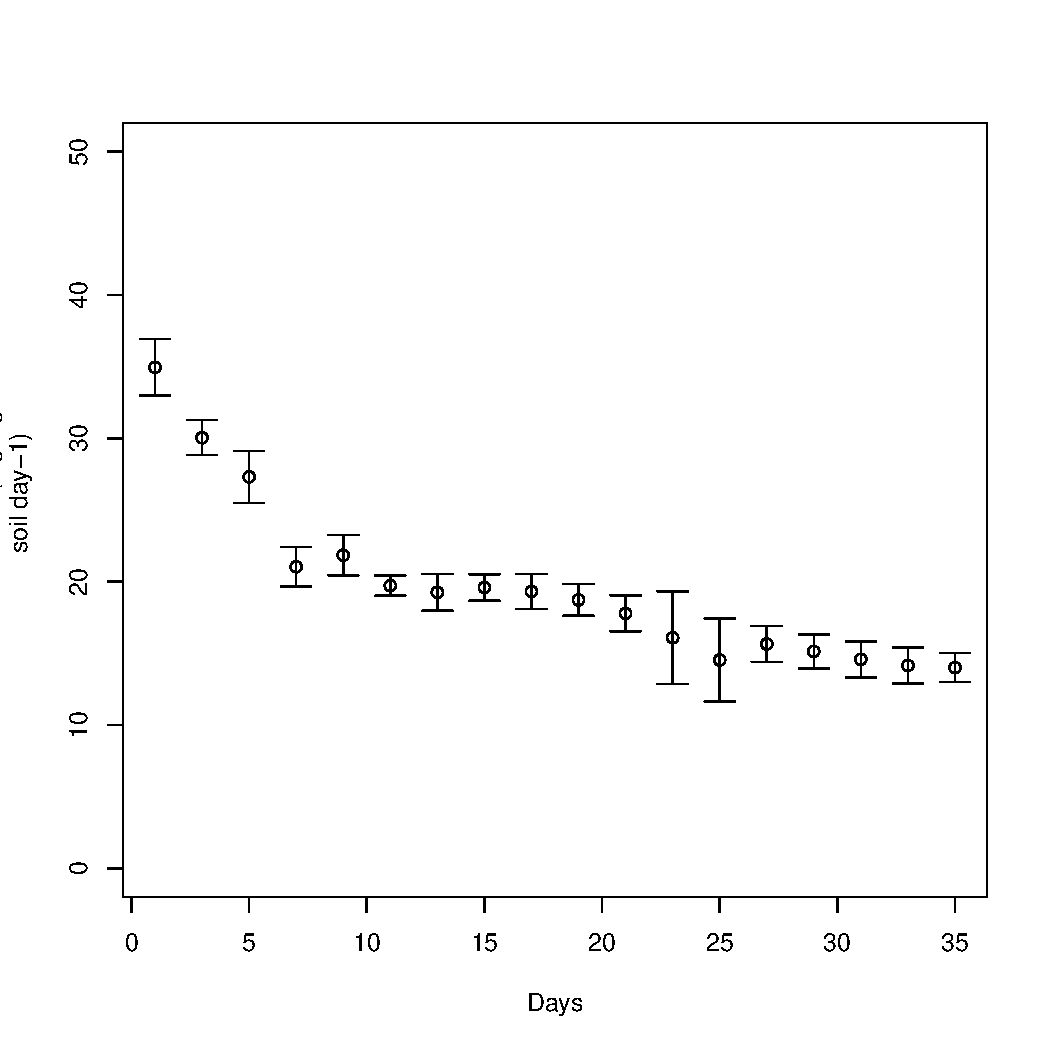
\includegraphics[width=\maxwidth]{figure/unnamed-chunk-5-1} 

\end{knitrout}
  \caption{Cummulative evolved CO$_2$ from an incubation experiment with a boreal forest soil.}
  \label{fig:eCO2}
\end{figure}
%Assume that we have some reasons to expect a two-pool model with feedback of the form \citep{SierraGMD} would be appropriate.
%\begin{align} \label{Model}
%\frac{dC_1}{dt} &= I - k_1 C_1 + \alpha_{1,2} k_2 C_2 \notag \\
%\frac{dC_2}{dt} &= \alpha_{2,1} k_1 C_1 - k_2 C_2
%\end{align}
%To fit this model to our dataset we have to estimate the values of the decomposition rates $k_1$ and $k_2$ as well as the transfer coefficient to pool 2 from pool 1 ($\alpha_{2,1}$) and to pool 1 from pool 2 ($\alpha_{1,2}$). Given that the data comes from an incubation experiment, we assume that there are no inputs of carbon, so $I=0$. Additionally, we need a value for the partitioning coefficient for the two fractions $\gamma$, so $C_1 = C_{total} \gamma$, and $C_2 = C_{total} (1- \gamma)$. 
\subsection{Principal identifiability of the model}
Before we embroil ourselfes in technicalities we should think about the general possibility to identify the parameters from a single time line of the combined release of an yet unknown number of pools with yet unknown connections and outlets. 
We face several challenges, in particular we have to:
\begin{enumerate}
\item 
	\label{accuracy} Find a class of models that is large enough to contain a model, capable of reproducing the observed data. If the class is to small we will ``underfit'' our data and the model will be ``biased''.
\item 
	\label{identifiability} Find a number of parameters that is small enough to be actually determined unambigiously from the data. If we have parameters whose effects enhance or cancel the effects of other parameters the parameterized model will be ``overfitted'' and make (possibly extremely) misleading predictions for data not included in the training set. (In our case the predicted timeline of an overfitted model could meet all the measurements very well but be completely unreasonable in between or beyond the measurement times.)
\item 
	\label{independence} Make sure that the parameters can at least be tested independently by the optimization procedure. 
		(We refer here not to the desired independence of the parameters w.r.t (with respect to) the impact on the result as mentioned under \enumref{identifiability} but to the shape of the set of valid parameters. 
		For n parameters the algorithms that we will use except 
		n ranges and assume to be able to choose \emph{any} combination 
		of parameters out of this n-dimensional rectangular set to form a \emph{valid} model.
		E.g. an optimization algorithm that changes parameters independently should 
		not accidentally create a model that breakes mass conservation or produces negative fluxes.
		\SoilR allows many ways to specify models, including functions whose arguments include matrices whose parameters are \emph{not} independent.
		Since it allways checks that the specified model is a valid compartmental system, it would actually stop the optimization procedure from trying 
		unreasonable parameters.)
\end{enumerate}
We will start with the simplest model that fulfills conditions \enumref{identifiability} and \enumref{independence} and extend it to improve the degree of accuracy until we are either satisfied or more likely can no longer guarantee \enumref{identifiability}.
Note that the search for accurate and identifyable soil models is an open research question \cite{Sierra2015SBB}. 
The possible answers are limited only by your igenuity and more severly by the availability of data as the example will demonstrate.
%If we find a subset of parametes with similar or reverse effects on the model prediction we can not hope to uniquely identify them. 
%In our example this is indeed the case since for a given set of parameters we can find another symmetric configuration. (Exchange the values of $\gamma_1,k_1,\alpha_{2,1}$ and  $\gamma_2,k_2,\alpha_{1,2}$.) In this light the goal to determine all five parameters appears overly ambitious and the numerical results confirm this. We will therefore have to reduce the number of parameters.
%To break the symmetrie we remove the flux from pool 2 to pool 1 (represented by the parameter $\alpha_{1,2}$).  Numerical experiments show that this is still too ambitious. The algorithms compute very erratic results and get stuck in  local minima. It turns out that we can estimate only two paramters confidently. We choose the decomposition rate $k_{1}$ of the first pool and  $\alpha_{2,1}$.
%
%The model \eqref{Model} is implemented in \SoilR by the function {\tt TwopFeedbackModel}. 
%We want to find the best set of parameters that fit the data using classical optimization using the \FME \, package \citep{Soetaert}. For this, we need to create a function that takes arbitrary values of the parameters of the model, creates a model in \SoilR, calculates the daily respiration flux, and returns the output consistent with \FME \, requirements. We also need to create a vector of time steps in days and give the total amount of carbon in the soil at the begining of the experiment (soil dry weigh times the average C concentration from three replicates, units in g C). 
%Furthermore we have to ensure that the parameters tested by the optimization algorithms constitute valid models. 
The \FME function we want to use is {\tt modFit}. Our first attempt to model the data is a one pool model with a constant decomposition rate k.
\begin{knitrout}
\definecolor{shadecolor}{rgb}{0.969, 0.969, 0.969}\color{fgcolor}\begin{kframe}
\begin{alltt}
\hlstd{days}\hlkwb{=}\hlkwd{seq}\hlstd{(}\hlnum{0}\hlstd{,}\hlnum{35}\hlstd{)}
\hlcom{#C concentration * 450 g soil}
\hlstd{Ctotal}\hlkwb{=}\hlkwd{mean}\hlstd{(}\hlkwd{c}\hlstd{(}\hlnum{0.04683975}\hlstd{,} \hlnum{0.04703255}\hlstd{,} \hlnum{0.04687287}\hlstd{))}\hlopt{*}\hlnum{450}
\hlcom{#Changed units}
\hlstd{BorealCO2}\hlkwb{=}\hlkwd{data.frame}\hlstd{(}
  \hlkwc{time}\hlstd{=BorealCO2[,}\hlnum{1}\hlstd{],}
  \hlstd{BorealCO2[,}\hlnum{2}\hlopt{:}\hlnum{3}\hlstd{]}\hlopt{*}\hlnum{1e-06}\hlopt{*}\hlstd{Ctotal}
\hlstd{)}

\hlstd{eCO2func}\hlkwb{=}\hlkwa{function}\hlstd{(}\hlkwc{pars}\hlstd{)\{}
  \hlstd{k1}\hlkwb{=}\hlstd{pars[}\hlnum{1}\hlstd{]}
  \hlstd{k2}\hlkwb{=}\hlnum{1e-4}\hlopt{*}\hlstd{k1}
  \hlstd{alpha}\hlkwb{=}\hlstd{pars[}\hlnum{2}\hlstd{]}
  \hlstd{gamma}\hlkwb{=}\hlnum{.0001}
  \hlstd{mod}\hlkwb{=}\hlkwd{TwopFeedbackModel}\hlstd{(}
    \hlkwc{t}\hlstd{=days}
    \hlstd{,}\hlkwc{ks}\hlstd{=}\hlkwd{c}\hlstd{(k1,k2)}
    \hlstd{,}\hlkwc{a21}\hlstd{=alpha}
    \hlstd{,}\hlkwc{a12}\hlstd{=}\hlnum{0}
    \hlstd{,}\hlkwc{C0}\hlstd{=Ctotal}\hlopt{*}\hlkwd{c}\hlstd{(gamma,}\hlnum{1}\hlopt{-}\hlstd{gamma)}
    \hlstd{,}\hlkwc{In}\hlstd{=}\hlnum{0}
    \hlstd{,}\hlkwc{pass}\hlstd{=}\hlnum{TRUE}
  \hlstd{)}
  \hlstd{Rt}\hlkwb{=}\hlkwd{getReleaseFlux}\hlstd{(mod)}
  \hlkwd{return}\hlstd{(}\hlkwd{data.frame}\hlstd{(}\hlkwc{time}\hlstd{=days,}\hlkwc{eCO2}\hlstd{=}\hlkwd{rowSums}\hlstd{(Rt)))}
\hlstd{\}}
\end{alltt}
\end{kframe}
\end{knitrout}

Notice that our function, {\tt eCO2func}, requires a vector of parameters {\tt pars} with the values of the first decomposition rate in positions 1 and the values of the transfered proportion $\alpha_{2,1}$ in position 2. This function returns a {\tt data.frame} with two columns, time in days and the sum of the cummulative release for the two pools. 

The next step is to create a cost function according to \FME \, requirements. This cost function takes as arguments a function with the model, the set of observations, and a measure of the error in the observations. The function calculates sums of squared residuals from the model output and the observed data, which can be further minimized for optimization. 

\begin{knitrout}
\definecolor{shadecolor}{rgb}{0.969, 0.969, 0.969}\color{fgcolor}\begin{kframe}
\begin{alltt}
\hlstd{eCO2cost}\hlkwb{=}\hlkwa{function}\hlstd{(}\hlkwc{pars}\hlstd{)\{}
  \hlstd{modelOutput}\hlkwb{=}\hlkwd{eCO2func}\hlstd{(pars)}
  \hlkwd{return}\hlstd{(}\hlkwd{modCost}\hlstd{(}\hlkwc{model}\hlstd{=modelOutput,} \hlkwc{obs}\hlstd{=BorealCO2,} \hlkwc{err}\hlstd{=}\hlstr{"eCO2sd"}\hlstd{))}
\hlstd{\}}
\end{alltt}
\end{kframe}
\end{knitrout}

This function returns an object of class {\tt modCost}, which can be further used by \FME. 
We strongly recommend to to read \FME \, documentation for sensitivity and identifiability analyses. 
We will use the function {\tt modFit}.
It implements the optimization as an iterative process.
First the cost function will be evaluated on the initial parameter values.
Then the algorithm will try to guess new parameters, evaluate the cost function again and repeat this process until the cost is small enough or the number of permitted iterations exceeded. 
We can choose the optimization method ( Levenberg-Marquardt in the example ) which determines how
the algorithm arrives determines the next parameters.


\begin{knitrout}
\definecolor{shadecolor}{rgb}{0.969, 0.969, 0.969}\color{fgcolor}\begin{kframe}
\begin{alltt}
\hlstd{inipars}\hlkwb{=}\hlkwd{c}\hlstd{(} \hlnum{1}\hlopt{/}\hlnum{20} \hlstd{,}\hlnum{1}\hlopt{/}\hlnum{100}\hlstd{)}
\hlstd{up}\hlkwb{=}\hlkwd{c}\hlstd{(}\hlnum{1}\hlstd{,}\hlnum{1}\hlstd{)}
\hlstd{lo}\hlkwb{=}\hlkwd{c}\hlstd{(}\hlnum{0}\hlstd{,}\hlnum{0}\hlstd{)}

\hlstd{eCO2fit}\hlkwb{=}\hlkwd{modFit}\hlstd{(}
    \hlkwc{f}\hlstd{=eCO2cost}
    \hlstd{,}\hlkwc{p}\hlstd{=inipars}
    \hlstd{,}\hlkwc{method}\hlstd{=}\hlstr{"Marq"}
    \hlstd{,}\hlkwc{upper}\hlstd{=up}
    \hlstd{,}\hlkwc{lower}\hlstd{=lo}
\hlstd{)}
\end{alltt}
\end{kframe}
\end{knitrout}

To see the best set of parameter values found by the function we can type:
\begin{knitrout}
\definecolor{shadecolor}{rgb}{0.969, 0.969, 0.969}\color{fgcolor}\begin{kframe}
\begin{alltt}
\hlstd{eCO2fit}\hlopt{$}\hlstd{par}
\end{alltt}
\begin{verbatim}
## [1] 1.696373e-01 3.203139e-09
\end{verbatim}
\end{kframe}
\end{knitrout}

These set of parameters can be used now to run the model again and plot the obtained model against the observations

\begin{knitrout}
\definecolor{shadecolor}{rgb}{0.969, 0.969, 0.969}\color{fgcolor}\begin{kframe}
\begin{alltt}
\hlstd{fitmod}\hlkwb{=}\hlkwd{eCO2func}\hlstd{(eCO2fit}\hlopt{$}\hlstd{par)}
\end{alltt}
\end{kframe}
\end{knitrout}

\begin{figure}
  \centering
\begin{knitrout}
\definecolor{shadecolor}{rgb}{0.969, 0.969, 0.969}\color{fgcolor}\begin{kframe}
\begin{alltt}
\hlkwd{plot}\hlstd{(BorealCO2[,}\hlnum{1}\hlopt{:}\hlnum{2}\hlstd{],} \hlkwc{xlab}\hlstd{=}\hlstr{"Days"}\hlstd{,} \hlkwc{ylab}\hlstd{=}\hlstr{"Evolved CO2 (gC day-1)"}\hlstd{,}\hlkwc{ylim}\hlstd{=}\hlkwd{c}\hlstd{(}\hlnum{0}\hlstd{,}\hlnum{9e-04}\hlstd{))}
\hlkwd{arrows}\hlstd{(BorealCO2[,}\hlnum{1}\hlstd{],BorealCO2[,}\hlnum{2}\hlstd{]}\hlopt{-}\hlstd{BorealCO2[,}\hlnum{3}\hlstd{],BorealCO2[,}\hlnum{1}\hlstd{],}
       \hlstd{BorealCO2[,}\hlnum{2}\hlstd{]}\hlopt{+}\hlstd{BorealCO2[,}\hlnum{3}\hlstd{],}\hlkwc{code}\hlstd{=}\hlnum{3}\hlstd{,}\hlkwc{angle}\hlstd{=}\hlnum{90}\hlstd{,}\hlkwc{length}\hlstd{=}\hlnum{0.1}\hlstd{)}
\hlkwd{lines}\hlstd{(fitmod)}
\end{alltt}
\end{kframe}
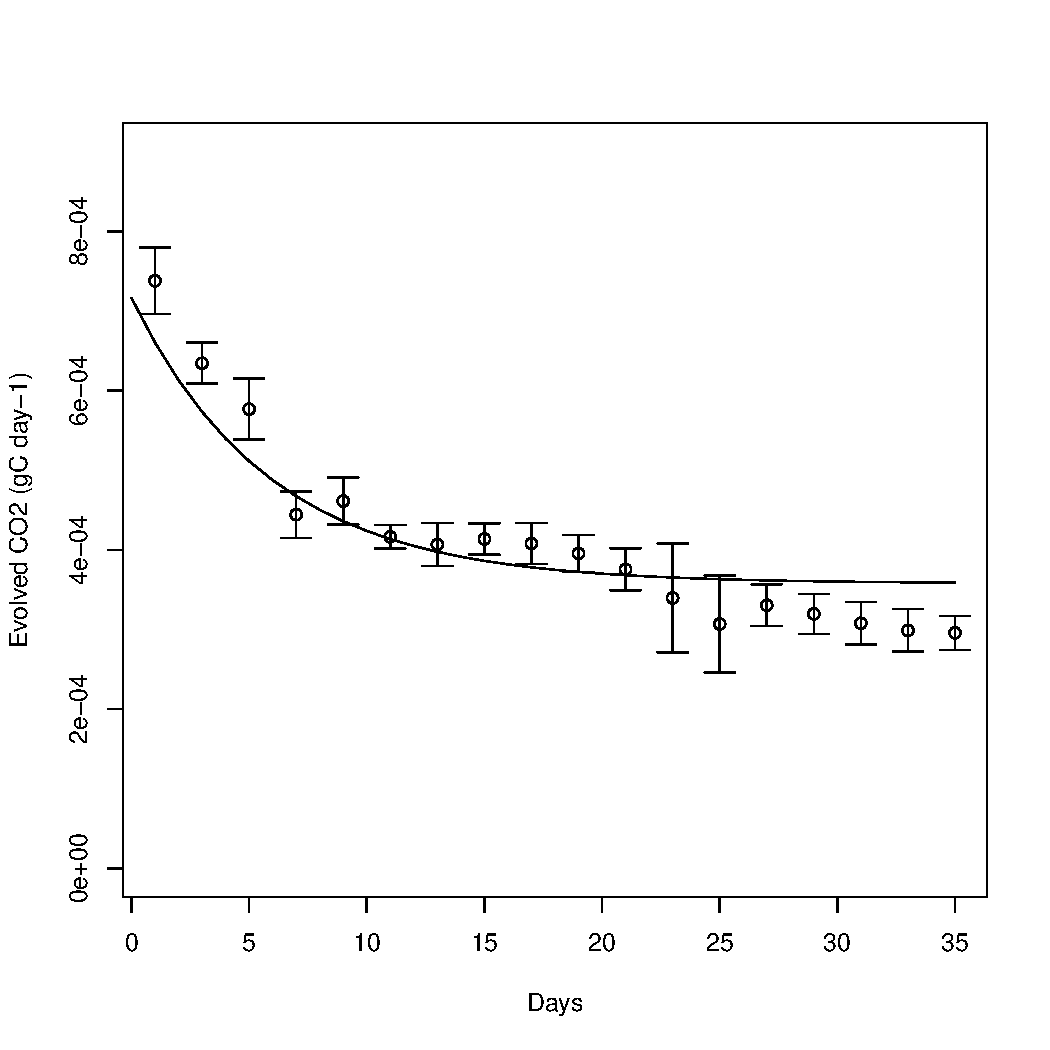
\includegraphics[width=\maxwidth]{figure/unnamed-chunk-11-1} 

\end{knitrout}
  \caption{Best fit curve and observed data of CO2 evolved from an incubation experiment.}
  \label{fig:fit}
\end{figure}

The results from this optimization can be used for Bayesian parameter estimation with \FME. For details about the procedure please see \citet{Soetaert}. In our example, we need first to extract the variance from the prior optimization and used as the initial variance in the Bayesian procedure and to determine the {\it jump}, a value that determines how much a new parameter set is deviated from the old one. To avoid long compiling times in \SoilR \,  we only use 1000 iterations in this example, but this number can be much larger to guarantee convergence of the chains. 



The results of the MCMC procedure can be obtained with the function {\tt summary()}. The output gives the mean, standard deviation, min and max, and 25\% quantiles for all parameter values. It also produces summary statistics for the variance of the observed variable. 


\begin{knitrout}
\definecolor{shadecolor}{rgb}{0.969, 0.969, 0.969}\color{fgcolor}\begin{kframe}
\begin{alltt}
\hlkwd{summary}\hlstd{(eCO2mcmc)}
\end{alltt}
\begin{verbatim}
##               p1           p2    var_eCO2
## mean 0.171720039 4.618881e-03 1.90553e-09
## sd   0.004700158 5.383253e-03 0.00000e+00
## min  0.158077194 1.860336e-09 1.90553e-09
## max  0.188593651 3.467826e-02 1.90553e-09
## q025 0.168401008 6.690192e-04 1.90553e-09
## q050 0.171847915 2.996371e-03 1.90553e-09
## q075 0.175018284 6.496190e-03 1.90553e-09
\end{verbatim}
\begin{alltt}
\hlstd{sR1}\hlkwb{=}\hlkwd{sensRange}\hlstd{(}\hlkwc{func}\hlstd{=eCO2func,} \hlkwc{parInput}\hlstd{=eCO2mcmc}\hlopt{$}\hlstd{par)}
\end{alltt}
\end{kframe}
\end{knitrout}

A plot with the posterior distribution of the obtained parameter values can be obtained with function {\tt pairs} (Figure \ref{fig:mcmc})

\begin{figure}
  \centering
\begin{knitrout}
\definecolor{shadecolor}{rgb}{0.969, 0.969, 0.969}\color{fgcolor}\begin{kframe}
\begin{alltt}
\hlkwd{pairs}\hlstd{(eCO2mcmc)}
\end{alltt}
\end{kframe}
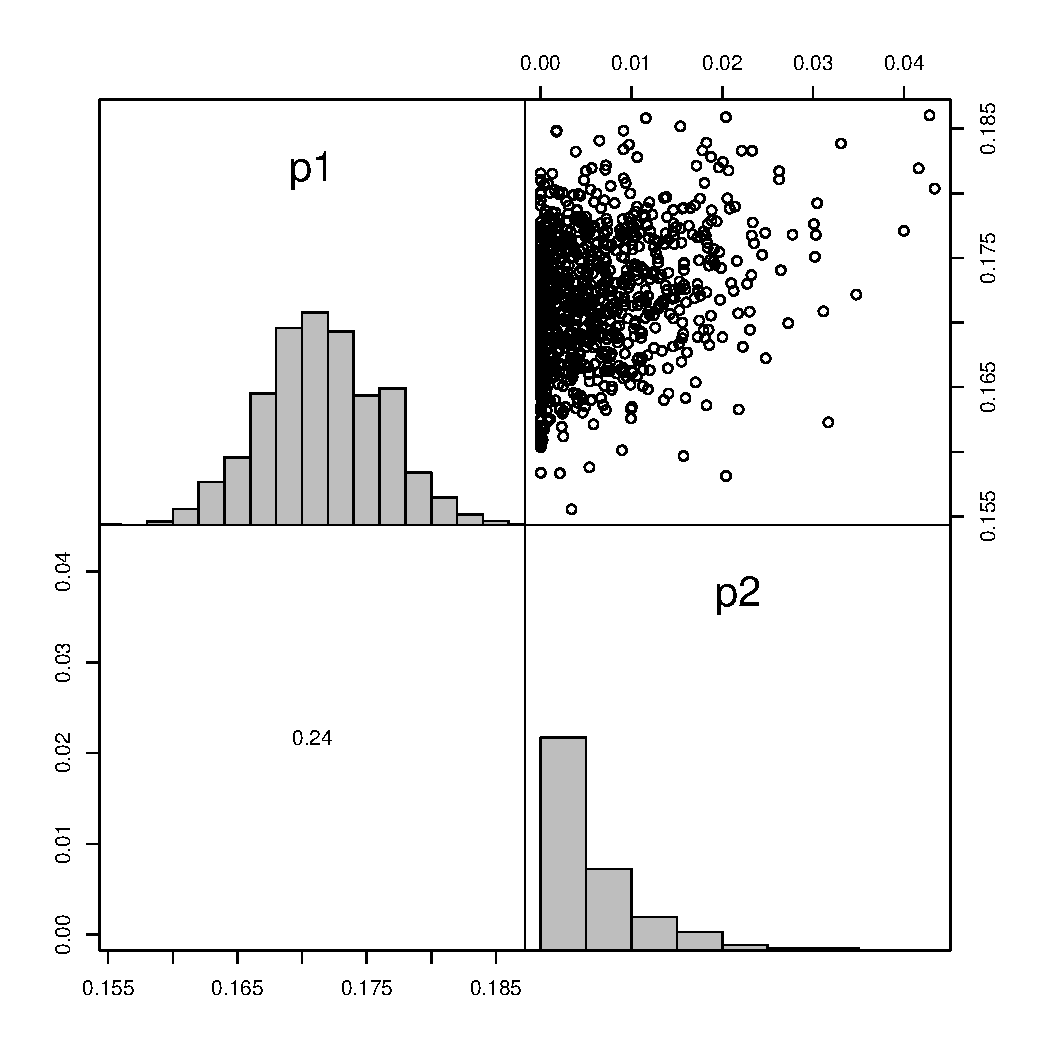
\includegraphics[width=\maxwidth]{figure/unnamed-chunk-14-1} 

\end{knitrout}
  \caption{Histogram and scatter plots of the values obtained from the Markov chain Monte Carlo procedure.}
  \label{fig:mcmc}
\end{figure}

For model prediction, it is also possible to use \FME \, and function {\tt sensRange} to obtain a graph of the model prediction with uncertainty ranges (Figure \ref{fig:sensRange}).

\begin{figure}
  \centering
\begin{knitrout}
\definecolor{shadecolor}{rgb}{0.969, 0.969, 0.969}\color{fgcolor}\begin{kframe}
\begin{alltt}
\hlstd{predRange}\hlkwb{=}\hlkwd{sensRange}\hlstd{(}\hlkwc{func}\hlstd{=eCO2func,} \hlkwc{parInput}\hlstd{=eCO2mcmc}\hlopt{$}\hlstd{par)}
\hlkwd{plot}\hlstd{(}\hlkwd{summary}\hlstd{(predRange),}\hlkwc{ylim}\hlstd{=}\hlkwd{c}\hlstd{(}\hlnum{0}\hlstd{,}\hlnum{9e-04}\hlstd{),}\hlkwc{xlab}\hlstd{=}\hlstr{"Days"}\hlstd{,}
     \hlkwc{ylab}\hlstd{=}\hlstr{"Evolved CO2 (g C day-1)"}\hlstd{,}\hlkwc{main}\hlstd{=}\hlstr{""}\hlstd{)}
\hlkwd{points}\hlstd{(BorealCO2)}
\hlkwd{arrows}\hlstd{(BorealCO2[,}\hlnum{1}\hlstd{],BorealCO2[,}\hlnum{2}\hlstd{]}\hlopt{-}\hlstd{BorealCO2[,}\hlnum{3}\hlstd{],BorealCO2[,}\hlnum{1}\hlstd{],}
       \hlstd{BorealCO2[,}\hlnum{2}\hlstd{]}\hlopt{+}\hlstd{BorealCO2[,}\hlnum{3}\hlstd{],}\hlkwc{code}\hlstd{=}\hlnum{3}\hlstd{,}\hlkwc{angle}\hlstd{=}\hlnum{90}\hlstd{,}\hlkwc{length}\hlstd{=}\hlnum{0.1}\hlstd{)}
\end{alltt}
\end{kframe}
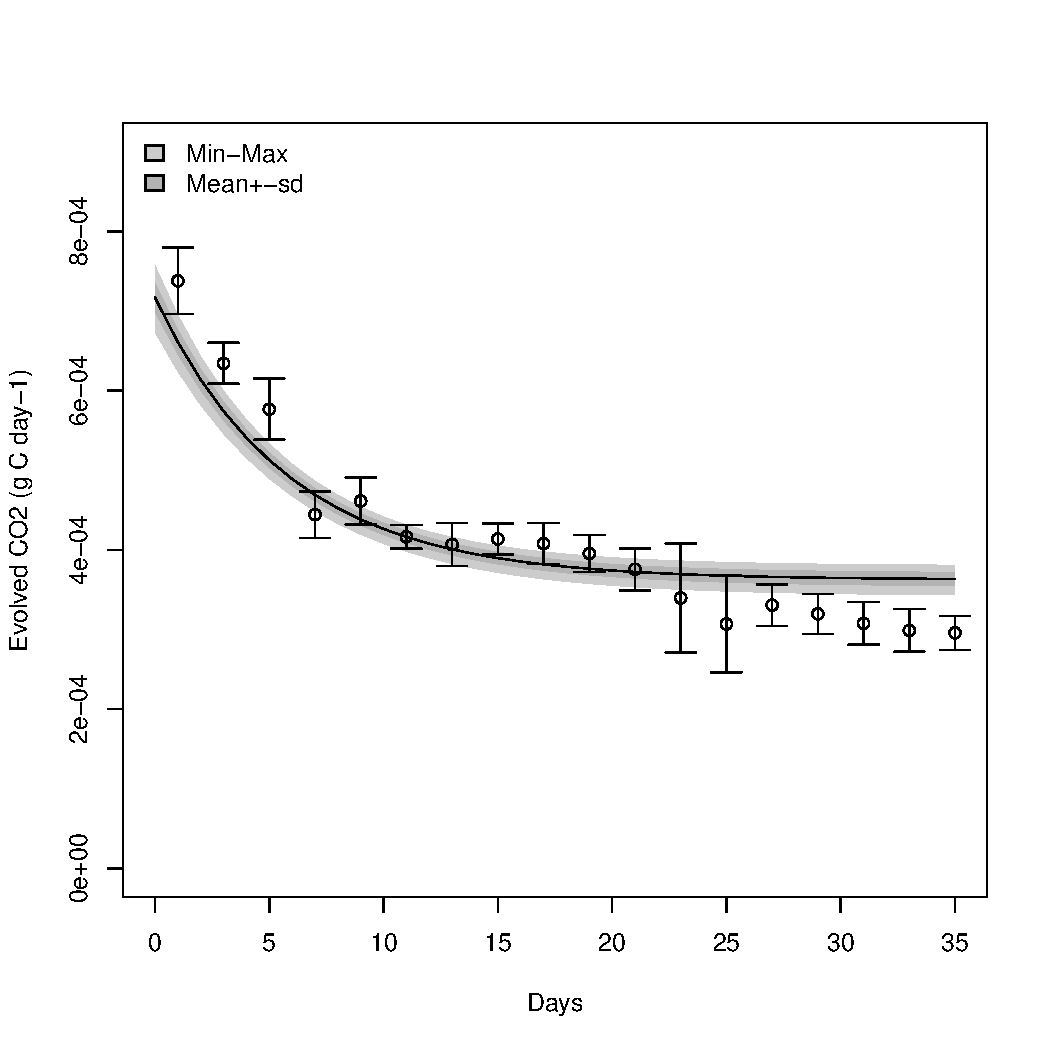
\includegraphics[width=\maxwidth]{figure/unnamed-chunk-15-1} 

\end{knitrout}
  \caption{Model predictions using the set of parameters obtained from the MCMC procedure.}
  \label{fig:sensRange}
\end{figure}

\clearpage
It is now obvious from this example that the workhorse of the parameter estimation procedure is the package \FME \, of \citet{Soetaert}. The main important task to learn about \SoilR \, is how to set up the function that runs the model and obtains the variable of interest.  

\section*{Example 2: Radiocarbon in respired CO$_2$}
\SoilR \, can also calculate the amount of radiocarbon in soils or in respired CO$_2$. Here, we take as an example a series of observations of radiocarbon in respired CO$_2$ conducted at Harvard Forest, USA. The dataset is also included in \SoilR, and is visualized in Figure \ref{fig:radiocarbondata}.

\begin{figure}
  \centering
\begin{knitrout}
\definecolor{shadecolor}{rgb}{0.969, 0.969, 0.969}\color{fgcolor}\begin{kframe}


{\ttfamily\noindent\color{warningcolor}{\#\# Warning in title(...): font metrics unknown for Unicode character U+2030}}

{\ttfamily\noindent\color{warningcolor}{\#\# Warning in title(...): conversion failure on '(‰)' in 'mbcsToSbcs': dot substituted for <e2>}}

{\ttfamily\noindent\color{warningcolor}{\#\# Warning in title(...): conversion failure on '(‰)' in 'mbcsToSbcs': dot substituted for <80>}}

{\ttfamily\noindent\color{warningcolor}{\#\# Warning in title(...): conversion failure on '(‰)' in 'mbcsToSbcs': dot substituted for <b0>}}

{\ttfamily\noindent\color{warningcolor}{\#\# Warning in title(...): font metrics unknown for Unicode character U+2030}}

{\ttfamily\noindent\color{warningcolor}{\#\# Warning in title(...): conversion failure on '(‰)' in 'mbcsToSbcs': dot substituted for <e2>}}

{\ttfamily\noindent\color{warningcolor}{\#\# Warning in title(...): conversion failure on '(‰)' in 'mbcsToSbcs': dot substituted for <80>}}

{\ttfamily\noindent\color{warningcolor}{\#\# Warning in title(...): conversion failure on '(‰)' in 'mbcsToSbcs': dot substituted for <b0>}}

{\ttfamily\noindent\color{warningcolor}{\#\# Warning in title(...): conversion failure on '(‰)' in 'mbcsToSbcs': dot substituted for <e2>}}

{\ttfamily\noindent\color{warningcolor}{\#\# Warning in title(...): conversion failure on '(‰)' in 'mbcsToSbcs': dot substituted for <80>}}

{\ttfamily\noindent\color{warningcolor}{\#\# Warning in title(...): conversion failure on '(‰)' in 'mbcsToSbcs': dot substituted for <b0>}}\end{kframe}
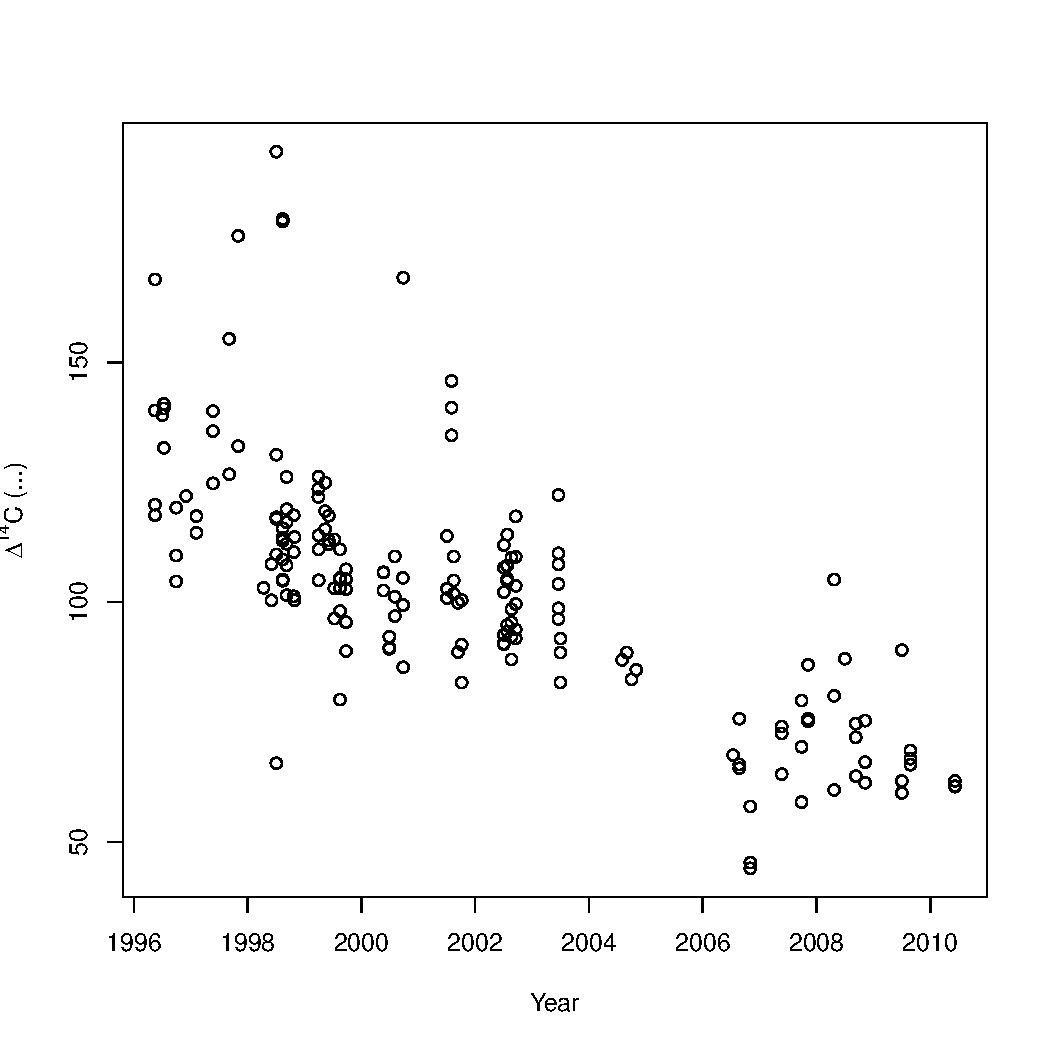
\includegraphics[width=\maxwidth]{figure/unnamed-chunk-16-1} 

\end{knitrout}
  \caption{$\Delta^{14}$C value of the respired CO$_2$ in a temperate broadleave forest at Harvard Forest, USA.}
  \label{fig:radiocarbondata}
\end{figure}

We are interested in fitting the following three-pool model to the data: 
\begin{equation} \label{eq:HarvardForestModel}
\frac{d {\bf C}(t)}{dt} = I \left( \begin{array}{c} \gamma_1 \\ \gamma_2 \\ 0 \end{array} \right) +
\left( \begin{array}{ccc}
-k_1 & 0 & 0 \\
a_{21} & -k_2 & 0 \\
a_{31} & 0 & -k_3
\end{array} \right)
\left( \begin{array}{c} C_1 \\ C_2 \\ C_3 \end{array} \right).
\end{equation}
where $\gamma_1$ and $\gamma_2$ are known. 
However the parameters $a_{21},a_{31},k_1,k_2,k_3 $ are not independent, which is a condition for the parameter estimation with FME.


For this task, we simply need to prepare a model object in \SoilR \, that can be further used by \FME \, for parameter estimation. 
The radiocarbon content of CO$_2$ in the atmosphere is necessary for running the model, because it informs us about the concentration and rate of radiocarbon input to the soil. For this example we will use the dataset {\tt C14Atm\_ NH} provided with \SoilR, but other provided datasets such as {\tt Hua2013} can also be used. 

First, we define the points in time to run the model from the atmospheric radicarbon dataset
\begin{knitrout}
\definecolor{shadecolor}{rgb}{0.969, 0.969, 0.969}\color{fgcolor}\begin{kframe}
\begin{alltt}
\hlstd{time}\hlkwb{=}\hlstd{C14Atm_NH}\hlopt{$}\hlstd{YEAR}
\hlstd{t_start}\hlkwb{=}\hlkwd{min}\hlstd{(time)}
\hlstd{t_end}\hlkwb{=}\hlkwd{max}\hlstd{(time)}
\end{alltt}
\end{kframe}
\end{knitrout}

To create the vector of input fluxes we need to create a new object of class {\tt InFlux}. For our particular model, input fluxes to the $C_1$ and $C_2$ pools are created by this command

\begin{knitrout}
\definecolor{shadecolor}{rgb}{0.969, 0.969, 0.969}\color{fgcolor}\begin{kframe}
\begin{alltt}
\hlstd{inputFluxes}\hlkwb{=}\hlkwd{InFlux}\hlstd{(} \hlkwd{c}\hlstd{(}\hlnum{270}\hlstd{,}\hlnum{150}\hlstd{,}\hlnum{0}\hlstd{))}
\end{alltt}
\end{kframe}
\end{knitrout}
assuming that pool 1 receives 270 gC m$^{2}$ yr$^{-1}$ and pool 2 150 gC m$^{2}$ yr$^{-1}$. 

The initial amount of carbon is created by aggregating the organic and mineral pools for this site reported in \citet{SierraBG}
\begin{knitrout}
\definecolor{shadecolor}{rgb}{0.969, 0.969, 0.969}\color{fgcolor}\begin{kframe}
\begin{alltt}
\hlstd{C0}\hlkwb{=}\hlkwd{c}\hlstd{(}\hlnum{390}\hlstd{,}\hlnum{220}\hlopt{+}\hlnum{390}\hlopt{+}\hlnum{1376}\hlstd{,}\hlnum{90}\hlopt{+}\hlnum{1800}\hlopt{+}\hlnum{560}\hlstd{)}
\end{alltt}
\end{kframe}
\end{knitrout}

We now write a function that creates a {\tt Model} object in \SoilR \, that takes as arguments a set of parameters and returns the 
$\Delta^{14}$C value of the respired carbon

%<<echo=false,results=hide>>=
\begin{knitrout}
\definecolor{shadecolor}{rgb}{0.969, 0.969, 0.969}\color{fgcolor}\begin{kframe}
\begin{alltt}
\hlstd{Fc}\hlkwb{=}\hlkwd{BoundFc}\hlstd{(C14Atm_NH,}\hlkwc{lag}\hlstd{=}\hlnum{0}\hlstd{,}\hlkwc{format}\hlstd{=}\hlstr{"Delta14C"}\hlstd{)}
\hlstd{np}\hlkwb{=}\hlnum{3}
\hlstd{Mod1}\hlkwb{<-}\hlkwa{function}\hlstd{(}\hlkwc{ks}\hlstd{,}\hlkwc{pass}\hlstd{=}\hlnum{TRUE}\hlstd{)\{}
  \hlstd{At}\hlkwb{=}\hlkwd{ConstLinDecompOp}\hlstd{(}
       \hlkwc{internal_flux_rates}\hlstd{=}\hlkwd{c}\hlstd{(}\hlstr{"1_to_2"}\hlstd{=ks[[}\hlnum{4}\hlstd{]],}\hlstr{"1_to_3"}\hlstd{=ks[[}\hlnum{5}\hlstd{]])}
      \hlstd{,}\hlkwc{out_flux_rates}\hlstd{=}\hlkwd{c}\hlstd{(}\hlstr{"1"}\hlstd{=ks[[}\hlnum{1}\hlstd{]],}\hlstr{"2"}\hlstd{=ks[[}\hlnum{2}\hlstd{]],}\hlstr{"3"}\hlstd{=ks[[}\hlnum{3}\hlstd{]])}
      \hlstd{,}\hlkwc{numberOfPools} \hlstd{= np}

  \hlstd{)}
  \hlstd{mod}\hlkwb{=}\hlkwd{GeneralModel_14}\hlstd{(}
        \hlkwc{t}\hlstd{=time,}
        \hlkwc{A}\hlstd{=At,}
        \hlkwc{ivList}\hlstd{=C0,}
        \hlkwc{initialValF}\hlstd{=}\hlkwd{ConstFc}\hlstd{(}\hlkwd{rep}\hlstd{(}\hlnum{0}\hlstd{,}\hlnum{3}\hlstd{),}\hlstr{"Delta14C"}\hlstd{),}
        \hlkwc{inputFluxes}\hlstd{=inputFluxes,}
        \hlkwc{inputFc}\hlstd{=Fc,}
        \hlkwc{pass}\hlstd{=}\hlnum{TRUE}
  \hlstd{)}
  \hlstd{R14t}\hlkwb{=}\hlkwd{getF14R}\hlstd{(mod)}
  \hlkwd{return}\hlstd{(}\hlkwd{data.frame}\hlstd{(}\hlkwc{time}\hlstd{=time,}\hlkwc{R14t}\hlstd{=R14t))}
\hlstd{\}}
\end{alltt}
\end{kframe}
\end{knitrout}

The observed data needs to be orginazed in a dataframe of the form
\begin{knitrout}
\definecolor{shadecolor}{rgb}{0.969, 0.969, 0.969}\color{fgcolor}\begin{kframe}
\begin{alltt}
\hlstd{DataR14t}\hlkwb{=}\hlkwd{cbind}\hlstd{(}\hlkwc{time}\hlstd{=HarvardForest14CO2[,}\hlnum{1}\hlstd{],}
               \hlkwc{R14t}\hlstd{=HarvardForest14CO2[,}\hlnum{2}\hlstd{],}
               \hlkwc{sd}\hlstd{=}\hlkwd{sd}\hlstd{(HarvardForest14CO2[,}\hlnum{2}\hlstd{]))}
\end{alltt}
\end{kframe}
\end{knitrout}


With all these elements ready, we can now use \FME \, for the parameter optimization procedure. We will avoid a detailed explanation and present in the following the creation of the cost function, the initial optimization, and the final Bayesian parameter estimation. 

\begin{knitrout}
\definecolor{shadecolor}{rgb}{0.969, 0.969, 0.969}\color{fgcolor}\begin{kframe}


{\ttfamily\noindent\bfseries\color{errorcolor}{\#\# Error in modFit(f = R14tCost, p = c(0.1, 0.2, 0.3, 0.4, 0.5), lower = rep(0, : object 'nk' not found}}

{\ttfamily\noindent\bfseries\color{errorcolor}{\#\# Error in eval(expr, envir, enclos): object 'Fit' not found}}

{\ttfamily\noindent\bfseries\color{errorcolor}{\#\# Error in summary(Fit): object 'Fit' not found}}

{\ttfamily\noindent\bfseries\color{errorcolor}{\#\# Error in modMCMC(f = R14tCost, p = Fit\$par, niter = number\_of\_iterations, : object 'Fit' not found}}\end{kframe}
\end{knitrout}

The obtained posterior distributions of the parameters can now be assessed graphically (Figure \ref{fig:HFmcmc}). The final model with its uncertainty and how it compares to the data can now be shown(Figure \ref{fig:HFmodel}). 
\begin{figure}
  \centering
\begin{knitrout}
\definecolor{shadecolor}{rgb}{0.969, 0.969, 0.969}\color{fgcolor}\begin{kframe}
\begin{alltt}
\hlkwd{pairs}\hlstd{(MCMC,}\hlkwc{nsample}\hlstd{=}\hlkwd{floor}\hlstd{(number_of_iterations}\hlopt{/}\hlnum{4}\hlstd{))}
\end{alltt}


{\ttfamily\noindent\bfseries\color{errorcolor}{\#\# Error in pairs(MCMC, nsample = floor(number\_of\_iterations/4)): object 'MCMC' not found}}\end{kframe}
\end{knitrout}
  \caption{Posterior parameter distributions for the parameters of the model described by equation \ref{eq:HarvardForestModel}. p1= $k_1$, p2= $k_2$, p3= $k_4$, p4= $a_{21}$, p5= $a_{31}$. Numbers in the lower diagonal indicate the correlation coefficient between parameters.}
  \label{fig:HFmcmc}
\end{figure}


\begin{figure}
  \centering
\begin{knitrout}
\definecolor{shadecolor}{rgb}{0.969, 0.969, 0.969}\color{fgcolor}\begin{kframe}
\begin{alltt}
\hlcom{#The sensitivity range is calculated from the output of the MCMC}
\hlstd{sR}\hlkwb{=}\hlkwd{sensRange}\hlstd{(}\hlkwc{func}\hlstd{=Mod1,} \hlkwc{parInput}\hlstd{=MCMC}\hlopt{$}\hlstd{par)}
\end{alltt}


{\ttfamily\noindent\bfseries\color{errorcolor}{\#\# Error in sensRange(func = Mod1, parInput = MCMC\$par): object 'MCMC' not found}}\begin{alltt}
\hlkwd{par}\hlstd{(}\hlkwc{mar}\hlstd{=}\hlkwd{c}\hlstd{(}\hlnum{5}\hlstd{,}\hlnum{5}\hlstd{,}\hlnum{4}\hlstd{,}\hlnum{1}\hlstd{))}
\hlkwd{plot}\hlstd{(}\hlkwd{summary}\hlstd{(sR),}\hlkwc{xlim}\hlstd{=}\hlkwd{c}\hlstd{(}\hlnum{1950}\hlstd{,}\hlnum{2010}\hlstd{),}\hlkwc{ylim}\hlstd{=}\hlkwd{c}\hlstd{(}\hlnum{0}\hlstd{,}\hlnum{1000}\hlstd{),}\hlkwc{xlab}\hlstd{=}\hlstr{"Year"}\hlstd{,}
     \hlkwc{ylab}\hlstd{=}\hlkwd{expression}\hlstd{(}\hlkwd{paste}\hlstd{(Delta}\hlopt{^}\hlnum{14}\hlstd{,}\hlstr{"C "}\hlstd{,}\hlstr{"(\textbackslash{}u2030)"}\hlstd{)),}\hlkwc{main}\hlstd{=}\hlstr{""}\hlstd{)}
\end{alltt}


{\ttfamily\noindent\bfseries\color{errorcolor}{\#\# Error in summary(sR): object 'sR' not found}}\begin{alltt}
\hlkwd{points}\hlstd{(DataR14t,}\hlkwc{pch}\hlstd{=}\hlnum{20}\hlstd{)}
\end{alltt}


{\ttfamily\noindent\bfseries\color{errorcolor}{\#\# Error in plot.xy(xy.coords(x, y), type = type, ...): plot.new has not been called yet}}\begin{alltt}
\hlkwd{lines}\hlstd{(C14Atm_NH,}\hlkwc{col}\hlstd{=}\hlnum{4}\hlstd{)}
\end{alltt}


{\ttfamily\noindent\bfseries\color{errorcolor}{\#\# Error in plot.xy(xy.coords(x, y), type = type, ...): plot.new has not been called yet}}\end{kframe}
\end{knitrout}
  \caption{Predictions of respired radiocarbon values from the model of equation \ref{eq:HarvardForestModel} versus observations. Model predictions include uncertainty range for the mean $\pm$ standard deviation, and the minimum-maximum range. Radiocarbon concentration in the atmosphere is depicted in blue.}
  \label{fig:HFmodel}
\end{figure}


\clearpage
\section*{Acknowledgements}
We would like to thank Saadat Malghani for performing the laboratory incubation study. Susan E. Trumbore provided the radiocarbon data for Harvard Forest and gave important support and insights for the development of this project. Funding from the Max Planck Society. 

\begin{thebibliography}{9}
\bibitem[Schadel et al.(2013)]{Schadel} Sch{\"a}del, C., Y.~Luo, R.~David~Evans, S.~Fei, and S.~Schaeffer. 2013
\newblock Separating soil {CO$_2$} efflux into {C}-pool-specific decay rates
  via inverse analysis of soil incubation data. {\it Oecologia} \newblock 171: 721--732.

\bibitem[Sierra et al.(2015)]{Sierra2015SBB} Sierra, C.A., Saadatullah Malghani and  M.~M\"uller. 2015 
	\newblock{ Model structure and parameter identification of soil organic matter models} 
	\newblock {\em Soil Biology and Biochemistry}, 90: 197-203.

\bibitem[Sierra et al.(2012)]{SierraGMD} Sierra, C.A., M.~M\"uller, and S.~E. Trumbore. 2012. \newblock Models of soil organic matter decomposition: the {SoilR} package, version 1.0. \newblock {\em Geosci. Model Dev.}, 5: 1045--1060.

\bibitem[Sierra et al.(2012)]{SierraBG} Sierra, C.A., S.~E. Trumbore, E.~A. Davidson, S.~D. Frey, K.~E. Savage, and  F.~M. Hopkins. 2012.
\newblock Predicting decadal trends and transient responses of radiocarbon storage and fluxes in a temperate forest soil.
\newblock {\em Biogeosciences}, 9: 3013--3028.

\bibitem[Soetaert \& Petzoldt(2010)]{Soetaert} Soetaert K. and T.~Petzoldt. 2010. \newblock Inverse modelling, sensitivity and monte carlo analysis in R using   package FME. \newblock {\em Journal of Statistical Software}, 33: 1--28.

\end{thebibliography}

\end{document}
